% !TeX spellcheck = en_US


\chapter{Control Algorithms}


\section{Overview}

The whisker control algorithm is developed to reconstruct an object's contour by swiping along its surface.
The following key requirements were determined for the control model design:

\begin{enumerate}
    \item \textbf{Precise Contour Reconstruction:} The algorithm must accurately capture the local shape at the point of contact, ensuring that the detailed profile of the object is recorded.
    \item \textbf{Accurate Curve Following:} It must adeptly follow both smooth curves and sharp angles, all while maintaining an optimal whisker deflection. The constant whisker deflection is crucial to have a predictable and small whisker tip position resolution by the deflection model.
    \item \textbf{Robust Detachment Recovery:} Sudden changes in the object's geometry can cause the whisker to detach. The system is therefore designed to quickly detect such events and recover contact with minimal disruption.
    \item \textbf{Collision Avoidance:} Considering the platform's dimensions, the algorithm incorporates measures to prevent collisions with the object during contour tracking.
\end{enumerate}

\noindent \textbf{Assumptions:} The development of this control strategy is based on the following assumptions:
\begin{enumerate}
    \item The contour is captured in a 2D (xy) plane, meaning that both the platform and whiskers operate with planar motion.
    \item All objects are rigid and remain stationary during the contact process.
    \item Contact occurs exclusively at the tip of the whisker.
    \item Forces exerted by the whiskers do not significantly affect the platform's motion.
    \item The platform's absolute position in the world frame is continuously known.
    \item The initial trajectory of the platform ensures that at least one whisker will eventually come into contact with the object.
    \item Although multiple objects may be present, the system focuses on a single object at any given time.
\end{enumerate}

\noindent To meet these requirements, the control algorithm is implemented as a finite state machine (FSM) that sequences the following policies:

\begin{enumerate}
    \item \textbf{Swiping Policy:} The whisker performs a continuous swiping motion along the object's curve while maintaining an optimal deflection profile.
    \item \textbf{Retrieval Policy:} In the event of whisker detachment, this policy analyzes the detachment reason, re-establishes contact and resumes the swiping motion, ensuring the contour continuity.
    \item \textbf{Tunnelling Policy:} When operating between two surfaces, the algorithm maintains a centered trajectory, thereby ensuring balanced contact on both sides.
\end{enumerate}

This structured approach enables the control system to dynamically adapt to varying contact scenarios.


\section{Data Preprocessing}

\subsection{Control Algorithm Variables}

It is necessary to consider the variables of the control algorithm.
Inputs come from three main sources:
\begin{enumerate}
    \item \textbf{Platform Sensors:} Provide the platform's position, orientation, and whisker deflection.
    \item \textbf{Geometric Configuration:} Information such as whisker placement.
    \item \textbf{Algorithm Configuration:} Parameters like the whisker deflection threshold.
\end{enumerate}
The output variables define the target linear and angular velocities of the platform.
A summary of these variables is provided in Table~\ref{tab:variables}.

\newcommand{\branch}[3]{%
    \scalebox{0.75}{$\left\{
                         \begin{array}{@{}l@{\quad}l@{}}
                             #2, & \text{if } #1,\\[0.5em]
                             #3, & \text{otherwise.}
                         \end{array}
    \right.$}%
}


\begin{table}[htb]
    \centering
    \begin{tabular}{p{1cm} p{2.2cm} p{3cm} p{7.8cm}}
        \toprule
        \textbf{Name}                                        & \textbf{Values}                                                   & \textbf{Source}                                         & \textbf{Description}                                                                                                        \\
        \midrule
        \multicolumn{4}{l}{\textbf{Control Inputs: Platform}} \\
        \midrule
        \(^{\mathrm{w}}\boldsymbol{r}^{t}\)                  & \(\mathbb{R}^2, [x, y]^\mathrm{T}\)                               & Measured                                                & Radius vector in world coordinates.                                                                                         \\
        \(^{\mathrm{w}}\alpha^{t}\)                          & \(\mathbb{R}\)                                                    & Measured                                                & Yaw angle (orientation) in world coordinates.                                                                               \\
        \(v_{\mathrm{total}}\)                               & \(\mathbb{R}^{+}\)                                                & Configuration                                           & Total platform velocity.                                                                                                    \\
        \midrule
        \multicolumn{4}{l}{\textbf{Control Inputs: Whisker \boldsymbol{$i=\mathrm{l,r}$}}} \\
        \midrule
        \(\delta_{i}^{t}\)                                   & \([-\delta_{\mathrm{i, \mathrm{max}}},\delta_{i, \mathrm{max}}]\) & Measured                                                & Deflection due to contact forces.                                                                                           \\
        \(\alpha_{i}^{t}\)                                   & \(\mathbb{R}\)                                                    & \(^{\mathrm{w}}\alpha^{t} + \alpha_{i, \mathrm{body}}\) & Yaw angle (orientation) of the whisker base in world coordinates.                                                           \\
        \(orient_{i}^{t}\)                                   & \(\{-1, 0, 1\}\)                                                  & \(sgn(\delta_{i}^{t}) \cdot side_{i}\)                  & Valid swipe orientation with current deflection: \(-1\) for clockwise, \(0\) for undefined, and \(1\) for counterclockwise. \\
        \(side_{i}\)                                         & \(\{-1, 1\}\)                                                     & \(\branch{\alpha_{i,\mathrm{body}} < 0}{-1}{1}\)        & Platform side where the whisker is fixed, -1 is left and 1 is right                                                         \\
        \(\delta_{i, \mathrm{thr}}\)                         & \(\mathbb{R}^{+}\)                                                & Deflection Model                                        & Deflection threshold value for contact detection (\(\delta_{i, \mathrm{thr}}\ll\delta_{i, \mathrm{max}}\)).                 \\
        \(\delta_{i, \mathrm{target}}\)                      & \([-\delta_{\mathrm{i, max}},\delta_{i, \mathrm{max}}]\)          & Deflection Model                                        & Target deflection value for small reconstruction error.                                                                     \\
        \(\;^{\mathrm{w}}\boldsymbol{r}_{i, \mathrm{body}}\) & \(\mathbb{R}^2\)                                                  & Robot Geometry                                          & Offset from the platform center to the whisker base.                                                                        \\
        \(\alpha_{i, \mathrm{body}}\)                        & \([-\pi,\pi)\)                                                    & Robot Geometry                                          & Angle for whisker placement relative to the platform.                                                                       \\
        \midrule
        \multicolumn{4}{l}{\textbf{Control Outputs}} \\
        \midrule
        \(^{\mathrm{w}}\boldsymbol{v}^{t}\)                  & \(\mathbb{R}^2, [v_x, v_y]^\mathrm{T}\)                           & --                                                      & Linear velocity vector in world coordinates.                                                                                \\
        \(^{\mathrm{w}}\omega^{t}\)                          & \(\mathbb{R}\)                                                    & --                                                      & Angular velocity (yaw) in world coordinates.                                                                                \\
        \bottomrule
    \end{tabular}
    \caption{Overview of input and output variables used in the control system.}
    \label{tab:variables}
\end{table}

\subsection{Deflection Smoothing}

The measured whisker deflection \(\delta_{i}^{t}\) is noisy due to vibrations and transient disturbances.
To reduce this noise, a low-pass Butterworth filter is applied.
The filter is initially seeded with the neutral deflection and updated with each new measurement.

\subsection{Deflection Model}

A 5th-degree polynomial is fitted to calibration data to model whisker deflection.
This model mirrors the deflection offset from the neutral position and clips the result based on the whisker's half-circle limit.
The deflection model is shown in Figure~\ref{fig:deflection_profile}.

\begin{figure}[htb]
    \centering
    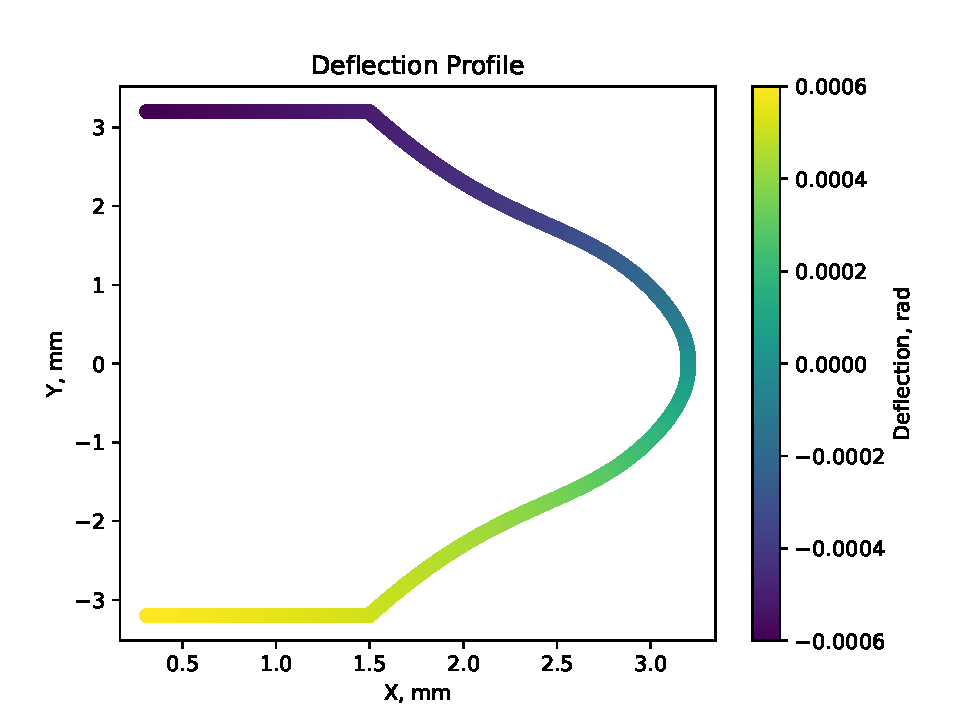
\includegraphics[width=0.8\textwidth]{figures/deflection_profile}
    \caption{Deflection Profile Model.}
    \label{fig:deflection_profile}
\end{figure}


\section{Body Motion Control}

Each control policy produces a target position for either the platform body or the whisker, which is then executed by the actuators.
To achieve accurate motion, the body motion control algorithm computes the necessary linear and angular velocities to reach the desired position.
A PID controller is used to generate the target angular velocity based on the difference between the current and desired orientations.
Meanwhile, the linear velocity is maintained at a constant magnitude, so that the resulting velocity vector is directly determined by the desired direction (see Algorithm~\ref{alg:steer_platform}).
In cases where the target position is specified for the whisker rather than the body, the algorithm applies a coordinate transformation to adjust the linear velocity accordingly.
This transformation compensates for the offset between the whisker and the body frame, ensuring that the control command is executed correctly (see Algorithm~\ref{alg:steer_whisker}).


\begin{algorithm}[htb]
    \caption{Steer the Platform to Target Position and Orientation}
    \begin{algorithmic}[1]
        \State Require \(^{\mathrm{w}}\boldsymbol{r}^{t+1}\), \(\;^{\mathrm{w}}\alpha^{t+1}\)
        \State \(^{\mathrm{w}}\omega^{t+1} \gets \mathrm{PID}(\;^{\mathrm{w}}\alpha^{t+1} - \;^{\mathrm{w}}\alpha^{t})\)
        \State \(^{\mathrm{w}}\boldsymbol{v}^{t+1} \gets v_{\mathrm{total}} \cdot \dfrac{^{\mathrm{w}}\boldsymbol{r}^{t+1}}{\|^{\mathrm{w}}\boldsymbol{r}^{t+1}\|}\)
        \State Return \(^{\mathrm{w}}\boldsymbol{v}^{t+1}\), \(^{\mathrm{w}}\omega^{t+1}\)
    \end{algorithmic}
    \label{alg:steer_platform}
\end{algorithm}

\begin{algorithm}[htb]
    \caption{Steer Whisker to Target Position and Orientation}
    \begin{algorithmic}[1]
        \State Require \(^{\mathrm{w}}\boldsymbol{r}_{\mathrm{wsk}}^{t+1}\), \(^{\mathrm{w}}\alpha^{t+1}\)
        \State \((^{\mathrm{w}}\boldsymbol{v}^{t+1},\, ^{\mathrm{w}}\omega^{t+1}) \gets \mathrm{steer\_body}(\;^{\mathrm{w}}\boldsymbol{r}_{\mathrm{wsk}}^{t+1},\, ^{\mathrm{w}}\alpha^{t+1})\)
        \State \(^{\mathrm{w}}\boldsymbol{r}_{\mathrm{corr}} \gets [0,\,0,\,^{\mathrm{w}}\omega^{t+1}] \times \boldsymbol{r}_{\mathrm{wsk, body}}\) \Comment{Correct for whisker offset (pivot shift)}
        \State \(^{\mathrm{w}}\boldsymbol{v}^{t+1} \gets v_{\mathrm{total}} \cdot \dfrac{^{\mathrm{w}}\boldsymbol{v}^{t+1} + \,^{\mathrm{w}}\boldsymbol{r}_{\mathrm{corr}}}{\|^{\mathrm{w}}\boldsymbol{v}^{t+1} + \,^{\mathrm{w}}\boldsymbol{r}_{\mathrm{corr}}\|}\)
        \State Return \(^{\mathrm{w}}\boldsymbol{v}^{t+1}\), \(^{\mathrm{w}}\omega^{t+1}\)
    \end{algorithmic}
    \label{alg:steer_whisker}
\end{algorithm}


\section{Swiping Policy}

The swiping policy aims to produce a smooth motion of the whisker along the object's contour while collecting high-precision shape data.
To achieve this, the whisker must maintain an optimal deflection profile because the accuracy of the deflection model depends on the current deflection.
This requires a balance between accurately following the object's curvature and preserving the target deflection.
The idea is demonstrated in Algorithm~\ref{alg:swiping_policy}.
For contour following, a B-Spline is used to represent the object's contour by incorporating the latest whisker tip position at each control iteration:
\[
    r_j = \bigl(x_j,y_j\bigr), \quad j=0,\dots,n-1.
\]
The local contour is given by
\[
    S(u) = \sum_{j=0}^{n-1} r_j \, B_{j,k,t}(u),
\]
where \(B_{j,k,t}(u)\) denotes the B-Spline basis functions of degree \(k\) defined on the knot vector \(t\).
We parameterize the keypoints uniformly by setting
\[
    u_k = 1 + \frac{k}{n-1}, \quad k=0,1,\dots,n-1.
\]
This B-Spline formulation provides a smooth approximation of the object's contour while allowing local control over the curve shape.
The keypoint collection is marked with a yellow background in the algorithm.

The tangent at the end of the spline is then used to determine the desired whisker orientation (see the code highlighted in blue).
To account for the whisker's deflection, the target whisker base-tip offset is calculated from the deflection model and compared with the desired target deflection.
The resulting whisker position is derived as a weighted sum of the vector that minimizes the deflection error and ensures the spline following (marked green in code).
For transient conditions—when the whisker deflection is below a predefined threshold or the spline has not yet been constructed—the swiping policy retains the existing control values.

\begin{algorithm}[htb]
    \caption{Swiping Policy}
    \begin{algorithmic}[1]
        \State If \(|\delta_{\mathrm{wsk}}^{t}| < \delta_{\mathrm{wsk, thr}}\) Then \Comment{Check that the whisker touches the object}
        \State \quad Return \(\;^{\mathrm{w}}\boldsymbol{v}^{t}\), \(\;^{\mathrm{w}}\omega^{t}\)
        \State End If
        \State
        \State \colorbox{yellow!40}{\(\;^{\mathrm{s}}\boldsymbol{r}_{\mathrm{tip}}^{t} \gets \mathrm{wsk.defl\_model}(\delta_{\mathrm{wsk}}^{t})\)}
        \State \colorbox{yellow!40}{\(\;^{\mathrm{w}}\boldsymbol{r}_{\mathrm{tip}}^{t} \gets \;^{\mathrm{w}}\boldsymbol{r}^{t} + \;^{\mathrm{w}}\boldsymbol{r}_{\mathrm{wsk, body}} + \boldsymbol{R}_{xy}^{2}(\; ^{\mathrm{w}}\alpha_{\mathrm{wsk}}^{t}) \cdot \;^{\mathrm{s}}\boldsymbol{r}_{\mathrm{tip}}^{t}\)}
        \State \colorbox{yellow!40}{\(\mathrm{wsk.spline.add\_keypoint}(\;^{\mathrm{w}}\boldsymbol{r}_{\mathrm{tip}}^{t})\)}
        \State If not \(\mathrm{wsk.spline.has\_enough\_points()}\) Then \Comment{Check that the spline is complete}
        \State \quad Return \(\;^{\mathrm{w}}\boldsymbol{v}^{t}\), \(\;^{\mathrm{w}}\omega^{t}\)
        \State End If
        \State
        \State \colorbox{cyan!40}{\(\;^{\mathrm{w}}\boldsymbol{\tau}_{\mathrm{spline}}^{t} \gets \dfrac{\mathrm{wsk.spline}(u\mathord{=}u_{k1}) - \mathrm{wsk.spline}(u\mathord{=}u_{k0})}{\|\mathrm{wsk.spline}(u\mathord{=}u_{k1}) - \mathrm{wsk.spline}(u\mathord{=}u_{k0})\|}\)} \Comment{Object surface tangent}
        \State \colorbox{cyan!40}{\(\;^{\mathrm{w}}\theta_{\mathrm{spline}}^{t} \gets \mathrm{arctan2}(\;^{\mathrm{w}}\boldsymbol{\tau}_{\mathrm{spline}}^{t})\)} \Comment{Object surface angle}
        \State \colorbox{cyan!40}{\(\;^{\mathrm{w}}\alpha^{t+1} \gets \;^{\mathrm{w}}\theta_{\mathrm{spline}}^{t}\)}
        \State \(\;^{\mathrm{s}}\boldsymbol{r}_{\mathrm{tip, target}}^{t} \gets \mathrm{wsk.defl\_model}\big(\delta_{\mathrm{wsk, target}} \cdot \operatorname{sgn}(\delta_{\mathrm{wsk}}^{t})\big)\) \Comment{Desired whisker base-tip offset}
        \State \(\Delta\boldsymbol{r}_{tip}^{t} \gets \boldsymbol{R}_{xy}^{2}(\; ^{\mathrm{w}}\alpha_{\mathrm{wsk}}^{t}) \cdot (\;^{\mathrm{s}}\boldsymbol{r}_{\mathrm{tip, target}} - \;^{\mathrm{s}}\boldsymbol{r}_{\mathrm{tip}}^{t})\) \Comment{\(\scriptstyle (\forall{t} \;^{\mathrm{w}}\boldsymbol{v}^{t+1} \updownarrow \Delta\boldsymbol{r}_{\mathrm{tip}}^{t}) \implies \delta_{\mathrm{wsk}}^{t} \xrightarrow[t \to \infty]{} \delta_{\mathrm{wsk, target}}\)}
        \State \(\;^{\mathrm{s}}\boldsymbol{r}_{\mathrm{tip, neutral}} \gets \mathrm{wsk.defl\_model}(0)\) \Comment{Undeformed whisker base-tip offset}
        \State \colorbox{green!40}{\(w_{\mathrm{defl}}^{t} \gets \dfrac{\|\Delta\boldsymbol{r}_{\mathrm{tip}}^{t}\|}{\|\;^{\mathrm{s}}\boldsymbol{r}_{\mathrm{tip, target}} - \;^{\mathrm{s}}\boldsymbol{r}_{\mathrm{tip, neutral}}\|}\)}
        \State \colorbox{green!40}{\(\;^{\mathrm{w}}\boldsymbol{r}_{\mathrm{wsk}}^{t+1} \gets \;^{\mathrm{w}}\boldsymbol{r}_{\mathrm{wsk}}^{t} + w_{\mathrm{defl}}^{t} \cdot \dfrac{-\Delta\boldsymbol{r}_{\mathrm{tip}}^{t}}{\|\Delta\boldsymbol{r}_{\mathrm{tip}}^{t}\|} + (1 - w_{\mathrm{defl}}^{t}) \cdot \dfrac{\;^{\mathrm{w}}\boldsymbol{\tau}_{\mathrm{spline}}^{t}}{\|\;^{\mathrm{w}}\boldsymbol{\tau}_{\mathrm{spline}}^{t}\|}\)} \Comment{Weighted sum}
        \State \((\;^{\mathrm{w}}\boldsymbol{v}^{t+1}, \;^{\mathrm{w}}\omega^{t+1}) \gets \mathrm{steer\_wsk}(\;^{\mathrm{w}}\boldsymbol{r}_{\mathrm{wsk}}^{t+1},\;^{\mathrm{w}}\alpha^{t+1}\)
        \State Return \(\;^{\mathrm{w}}\boldsymbol{v}^{t+1}, \;^{\mathrm{w}}\omega^{t+1}\)
    \end{algorithmic}
    \label{alg:swiping_policy}
\end{algorithm}

The contour is reconstructed by sequentially connecting the spline keypoints.
The swiping motion stops when the latest keypoint is closer to the starting position than the distance between consecutive keypoints and when a predetermined trajectory length has been achieved.


\section{Retrieval Policy}

The retrieval policy re-establishes contact with the object when the whisker detaches, minimizing platform movement and resuming swiping as quickly as possible.
Detachment can occur due to:
\begin{enumerate}
    \item \textbf{Object Surface:} The curve's angle is too sharp for the whisker to follow.
    \item \textbf{Slippage:}
    \begin{enumerate}
        \item \textbf{Forward Slippage:} Occurs when the angle increases, but the whisker remains momentarily engaged due to traction.
        \item \textbf{Backward Slippage:} Occurs when an inadequate deflection profile leads to tension buildup.
    \end{enumerate}
\end{enumerate}

The main challenge is determining the actual object profile for continued navigation.
Since minor slippage is handled by the swiping policy, the focus here is on detachment due to the object's surface.
The expected contact angle ranges from approximately 10\textminus20\textdegree{} (as the whisker moves from the deflected position toward neutral) up to 180\textdegree.
A test point on the opposite side of the edge is used to determine the true edge angle, as the spline cannot be updated.

\subsection{Premise}
If the whisker remains detached beyond a predefined threshold, it is considered disengaged and the retrieval policy takes over from the swiping policy.

\subsubsection{Angle Resolution}
The angle resolution strategy operates as follows:
\begin{itemize}
    \item The whisker returns to a starting angle-detection position.
    \item It targets the nearest out of all potential contact point at a fixed distance from the last known position; the locus of such points is a circle.
    \item It moves sequentially from one candidate point to another, until the contact is established, as shown in Figure~\ref{fig:angle_retrieval}.
    For every candidate point on the circle, the whisker's yaw is adjusted so that it contacts the object at a predefined angle.
    The object's surface is assumed to be a straight line from edge to the candidate point.
    \item Once the contact is re-established, the edge angle is determined as an angle between the spline tangent before the detachment and the line connecting the edge and the contact point.
    The required deflection threshold to detect the contact is set high enough for the deflection model to have a sufficiently small error during the next step with such a deflection.
\end{itemize}

\begin{figure}[htb]
    \centering
    \begin{tikzpicture}[scale=2]
        \coordinate (E) at (0,0);
        \coordinate (X) at (2,0);
        \coordinate (Y) at ({2*cos(30)},{2*sin(30)});
        \coordinate (Yp) at ({2*cos(135)},{2*sin(135)});
        \coordinate (C) at ({cos(30)},{sin(30)});
        \coordinate (W) at ({cos(135)}, {sin(135)});
        \coordinate (T) at ({cos(135) - cos(135 - 90)}, {sin(135) - sin(135 - 90)});
        \coordinate (B) at ({cos(135) - 2*cos(135 - 90 + 20)}, {sin(135) - 2*sin(135 - 90 + 20)});

        \draw [blue, dotted] (E) circle (1);
        \draw (E) -- (X);
        \draw (E) -- (Y);
        \draw [green] (B) -- (W);
        \draw [blue, dashed] (E) -- (Yp);
        \draw [blue, dashed] (W) -- (T);

        % Mark the 30° angle at vertex B.
        \draw (0.5,0) arc (0:30:0.5);
        \node [above, yshift=5mm] at (0.8,0.15) {$\beta$};

        % Mark the platform movement.
        \draw[-{Stealth[red]}] (2,-0.5) -- (0,-0.5);

        % Label the points.
        \fill (X) circle (1pt) node[below right] {$X$};
        \fill (E) circle (1pt) node[below left] {$E$};
        \fill (Y) circle (1pt) node[above right] {$Y$};
        \fill (Yp) circle (1pt) node[above right] {$Y'$};
        \fill (W) circle (1pt) node[above left] {$W$};
        \fill (B) circle (1pt) node[above left] {$B$};
        \fill (T) circle (1pt) node[above left] {$T$};

    \end{tikzpicture}
    \caption{Angle Retrieval Strategy. Black $[XE]$, $[EY]$ \textemdash{} object surface, Green $[BW]$ \textemdash{} the whisker, Blue $[EY']$ \textemdash{} the potential adjacent surface of the edge and its tangent $[WT]$, Blue circle \textemdash{} the targeted contact points.}
    \label{fig:angle_retrieval}
\end{figure}

\subsection{Whisking Back to the Edge}
The whisker moves back along the opposite side of the edge by linearly steering towards the edge.
As the radius is small with respect to the length of the whisker, such trajectory doesn't affect the deflection much, and the deflection profile is therefore preserved.
The selected radius guarantees that the distance from the contact point to the edge is sufficient to construct a new spline and predict the edge angle reliably.

\subsection{Transition to Swiping}
After analyzing the opposite side, the whisker intentionally detaches and repositions.
It is repositioned with a slight overshoot of the target attachment angle to ensure proper alignment when contact is re-established.
The whisker then reverses the direction of movement to re-engage with the object.
Once the new spline is constructed on the opposite side, the control is transferred back to the swiping policy, thereby completing the retrieval maneuver.


\section{Tunneling Policy}

The tunneling policy ensures that the platform maintains a centered trajectory between two surfaces, which optimizes whisker contact on both sides.
The idea is demonstrated in Algorithm~\ref{alg:tunneling_policy}.
A midpoint spline is generated by computing keypoints defined as the midpoints between the left and right whisker contacts (yellow).
This B-Spline serves as a continuous reference for steering the platform through tunnel-like environments.
The target angle is determined by the tangent of the midpoint spline (cyan).
The target position is calculated as current position plus the weighted sum of the spline tangent and deflection “pull“ (green).
This pull evaluates the difference between the current and target deflections as a ratio for both whiskers and shows, whether the normal movement is needed to correct the deflection.

\begin{algorithm}
    \caption{Tunneling Policy Control}
    \label{alg:tunneling_policy}
    \begin{algorithmic}[1]
        \State \colorbox{yellow!40}{\(\;^{\mathrm{w}}\boldsymbol{r}_{\mathrm{tip, r}}^{t} \gets \;^{\mathrm{w}}\boldsymbol{r}^{t} + \;^{\mathrm{w}}\boldsymbol{r}_{\mathrm{r, body}} + \boldsymbol{R}_{xy}^{2}(\; ^{\mathrm{w}}\alpha_{\mathrm{r}}^{t}) \cdot \mathrm{r.defl\_model}(\delta_{\mathrm{r}}^{t})\)}
        \State \colorbox{yellow!40}{\(\;^{\mathrm{w}}\boldsymbol{r}_{\mathrm{tip, l}}^{t} \gets \;^{\mathrm{w}}\boldsymbol{r}^{t} + \;^{\mathrm{w}}\boldsymbol{r}_{\mathrm{l, body}} + \boldsymbol{R}_{xy}^{2}(\; ^{\mathrm{w}}\alpha_{\mathrm{l}}^{t}) \cdot \mathrm{l.defl\_model}(\delta_{\mathrm{l}}^{t})\)}
        \State \colorbox{yellow!40}{\(\mathrm{midpoint\_spline.add\_keypoint}\big((\;^{\mathrm{w}}\boldsymbol{r}_{\mathrm{tip, r}}^{t} + \;^{\mathrm{w}}\boldsymbol{r}_{\mathrm{tip, l}}^{t}) / 2\big)\)}
        \State If not \(\mathrm{midpoint\_spline.has\_enough\_points}\) Then Return \(\;^{\mathrm{w}}\boldsymbol{v}^{t}\), \(\;^{\mathrm{w}}\omega^{t}\) End If
        \State
        \State \colorbox{cyan!40}{\(\;^{\mathrm{w}}\boldsymbol{\tau}_{\mathrm{spline}}^{t} \gets \mathrm{midpoint\_spline}(u\mathord{=}1) - \mathrm{midpoint\_spline}(u\mathord{=}0)\)}
        \State \colorbox{cyan!40}{\(\;^{\mathrm{w}}\boldsymbol{n}_{\mathrm{spline}}^{t} \gets \boldsymbol{R}_{xy}^{2}(\pi/2 \cdot orient_\mathrm{r}^t)\cdot\;^{\mathrm{w}}\boldsymbol{\tau}_{\mathrm{spline}}^{t}\)}
        \State \colorbox{cyan!40}{\(\;^{\mathrm{w}}\theta_{\mathrm{spline}}^{t} \gets \mathrm{arctan2}(\;^{\mathrm{w}}\boldsymbol{\tau}_{\mathrm{spline}}^{t})\)}
        \State \colorbox{green!40}{\(\mathrm{pull_{total}} \gets \mathrm{clip}\big(\frac{\delta_{\mathrm{r}}^{t} - \delta_{\mathrm{r, target}}}{\delta_{\mathrm{r, target}}} - \frac{\delta_{\mathrm{l}}^{t} - \delta_{\mathrm{l, target}}}{\delta_{\mathrm{l, target}}},\mathrm{\min}\mathord{=}-1, \mathrm{\max}\mathord{=}1\big)\)}
        \State \colorbox{green!40}{\(\;^{\mathrm{w}}\boldsymbol{r}^{t+1} \gets \;^{\mathrm{w}}\boldsymbol{r}^{t} + \;^{\mathrm{w}}\boldsymbol{\tau}_{\mathrm{spline}}^{t} + \mathrm{pull_{total}}/2 \cdot \;^{\mathrm{w}}\boldsymbol{n}_{\mathrm{spline}}^{t}\)}
        \State \((\;^{\mathrm{w}}\boldsymbol{v}^{t+1}, \;^{\mathrm{w}}\omega^{t+1}) \gets steer\_body(\;^{\mathrm{w}}\boldsymbol{r}^{t+1},\;^{\mathrm{w}}\theta_{\mathrm{spline}}^{t})\)
        \State Return \(\;^{\mathrm{w}}\boldsymbol{v}^{t+1}, \;^{\mathrm{w}}\omega^{t+1}\)
    \end{algorithmic}
\end{algorithm}


\section{Finite State Machine}

The policies are specialized and only in combination can the whisker harness their full potential.
A finite state machine (FSM) is used to implement these policies, with each policy represented as a state.
Transitions occur when specific events arise, such as ``whisker has come into contact with the surface'' or ``whisker has become disengaged.''
The statechart of the FSM for the discussed policies is shown in \cref{fig:fsm}.

\begin{figure}[htb]
    \centering
    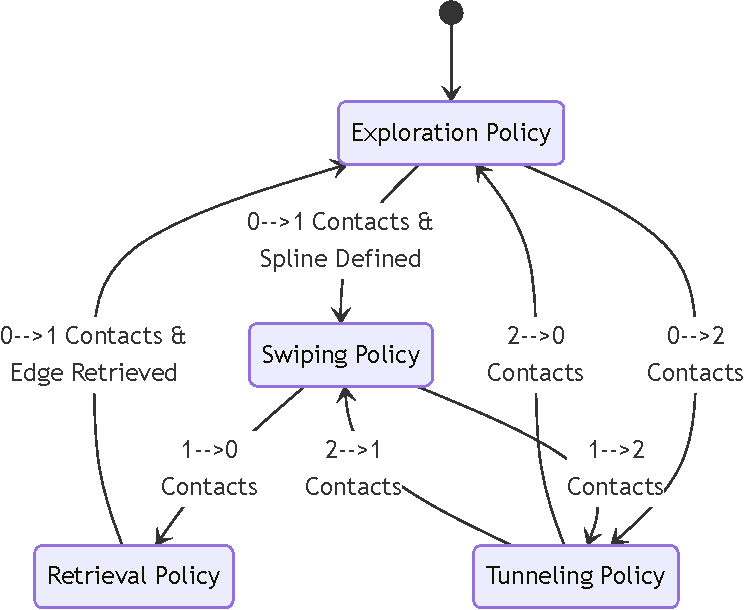
\includegraphics[width=0.8\textwidth]{figures/fsm}
    \caption{FSM diagram of the whisker control system. The diagram illustrates the various states (Exploring, Swiping, Tunneling, Retrieval, Whisking, Failure) and the transitions triggered by events such as contact establishment, detachment, and reattachment.}
    \label{fig:fsm}
\end{figure}


\section{Additional features}

Additional modifications can be applied to the control algorithm depending on the specific requirements of the task.

\subsection{Retrieval without Edge Reconstruction}

If the goal is to quickly analyze the object's surface without precise edge reconstruction, the whisking step in the retrieval policy can be skipped so that the angle resolution stage directly leads to swiping on the opposite side.

\subsection{Platform Tilt}

For improved stability during swiping (i.e. to handle sharper angles without separation), the platform can be tilted slightly toward the object.
This requires a simple modification of the body motion control algorithm by adjusting the target orientation by a small angle.
The tilt increases the duration of whisker contact with the surface, as the platform maintains its direction, which is beneficial given that the spline is constructed only at the contact point and cannot predict the future curve far away.

\subsection{Reverse Swiping}

If it is necessary for the platform to backtrack its path, the swiping policy can be modified to follow the spline in the reverse direction.
This is achieved by redefining the principal movement direction (normally aligned with the "nose" of the platform) in reverse mode.
Consequently, the body motion control algorithm computes the linear velocity using an oppositely offset yaw.
The retrieval policy is adjusted accordingly, as it depends solely on the position of the whisker base and is independent of the platform's overall orientation.

\subsection{Positioning of Whiskers at Different Angles}

Improving the adhesion of the whisker to the object can be achieved by positioning the whisker at an angle relative to the platform while maintaining the platform's tangential alignment with the object.
This approach follows the same principle as tilting, but preserves the platform's angle relative to the object.
This modification is particularly important in tunneling scenarios, where both whiskers must negotiate turns without becoming stuck.
When entering a tunnel, the first whisker contacts the surface, followed by the second whisker.
It is critical that the second whisker is positioned at an appropriate angle relative to the platform (typically slightly behind the main body).
If the whisker points directly in the direction of movement, it may insert into surface cavities and bend as if the platform were moving in the opposite direction, risking damage due to excessive deflection.
Positioning the whisker slightly backward prevents direct head-on contact with the tunnel wall.

\subsection{Integration of Multiple Whiskers on Each Side}

Multiple whiskers can be integrated on each side of the platform to:
\begin{itemize}
    \item Increase the precision of surface resolution.
    \item Enable single-shot swiping without the need for retrieval, as the retrieval radius is smaller than the distance between two whisker bases.
    \item Detect contacts at a wider range by extending the search space.
\end{itemize}


\section{Comparison to the Baseline}

\subsection{Baseline Algorithm}

The baseline algorithm from previous work implements the swiping policy as follows:
\begin{itemize}
    \item A Kalman filter is applied for preprocessing, using measurement noise covariance to estimate the whisker deflection offset.
    \item The swiping policy employs a single PID controller that takes the whisker deflection error as input and returns the desired velocity in the direction of the object (in the sensor frame).
    \item The total velocity is maintained, with the principal direction velocity in the local frame calculated as the complement to the velocity toward whisker compression or relaxation.
    \item The output velocity in the world frame is obtained by rotating the local frame velocity by the whisker tip spline tangent.
\end{itemize}
The underlying idea is that to track the surface, the whisker profile (i.e. its deflection) must remain constant; hence, the platform moves closer to the object when the whisker is too relaxed and moves away when it is too strained.

\subsection{Comparison to Baseline}

\subsubsection{Baseline Swiping Policy Evaluation}

\textbf{Pros:}
\begin{itemize}
    \item The whisker deflection offset is less susceptible to noise due to filtering.
    \item The swiping policy is straightforward and is designed to maintain a constant whisker profile.
\end{itemize}

\textbf{Cons:}
\begin{itemize}
    \item Filtering does not resolve the inherent noise or limitations of an ill-posed deflection model; subtle changes in whisker deflection that may be important for surface reconstruction can be lost.
    \item Maintaining a constant deflection profile ensures surface tracking but does not guarantee complete contour capture.
    \item The platform's velocity is relatively slow, and sudden changes in the principal direction—due to whisker slippage—can result in a 180° change in the spline direction, potentially causing reverse motion.
\end{itemize}

\subsubsection{Rectifying the Baseline Swiping Policy}
\begin{enumerate}
    \item To enhance reactivity, remove the Kalman filter and apply smoothing directly to the deflection signal (using the low-pass Butterworth filter described in Section~\ref{sec:deflection_smoothing}).
    \item Modify the swiping policy to balance the importance of following the spline with maintaining the deflection profile.
    \item Introduce a whisker orientation parameter (clockwise or counterclockwise) to prevent the whisker profile from deflecting in the opposite direction during control.
    This orientation is set upon initial contact with the surface and is preserved until the whisker disengages.
    It is employed in the calculation of the desired whisker base-tip offset.
\end{enumerate}

\subsection{Limitations of the Suggested Control Algorithm}
\begin{itemize}
    \item It does not take the platform dimensions into account to prevent non-whisker contacts.
    \item It requires parameter tuning (e.g., velocity, desired deflection, contact deflection threshold, PID parameters, etc.) to work properly.
    \item It is not failsafe in terms of whisker integrity, as extreme deflections are not directly forbidden.
    \item It does not allow for non-constant velocity and does not optimize the velocity for the environment.
    \item It can lead to situations in which the platform might get stuck (for instance, at the tunnel end, since the minimal space required for platform rotation without damaging the whisker is not calculated).
    \item There are other limitations imposed by the assumptions discussed earlier.
\end{itemize}
